\documentclass[]{book}
\usepackage{lmodern}
\usepackage{amssymb,amsmath}
\usepackage{ifxetex,ifluatex}
\usepackage{fixltx2e} % provides \textsubscript
\ifnum 0\ifxetex 1\fi\ifluatex 1\fi=0 % if pdftex
  \usepackage[T1]{fontenc}
  \usepackage[utf8]{inputenc}
\else % if luatex or xelatex
  \ifxetex
    \usepackage{mathspec}
  \else
    \usepackage{fontspec}
  \fi
  \defaultfontfeatures{Ligatures=TeX,Scale=MatchLowercase}
\fi
% use upquote if available, for straight quotes in verbatim environments
\IfFileExists{upquote.sty}{\usepackage{upquote}}{}
% use microtype if available
\IfFileExists{microtype.sty}{%
\usepackage{microtype}
\UseMicrotypeSet[protrusion]{basicmath} % disable protrusion for tt fonts
}{}
\usepackage[margin=1in]{geometry}
\usepackage{hyperref}
\hypersetup{unicode=true,
            pdftitle={R Best Practice},
            pdfauthor={Chad Goymer},
            pdfborder={0 0 0},
            breaklinks=true}
\urlstyle{same}  % don't use monospace font for urls
\usepackage{natbib}
\bibliographystyle{apalike}
\usepackage{color}
\usepackage{fancyvrb}
\newcommand{\VerbBar}{|}
\newcommand{\VERB}{\Verb[commandchars=\\\{\}]}
\DefineVerbatimEnvironment{Highlighting}{Verbatim}{commandchars=\\\{\}}
% Add ',fontsize=\small' for more characters per line
\usepackage{framed}
\definecolor{shadecolor}{RGB}{248,248,248}
\newenvironment{Shaded}{\begin{snugshade}}{\end{snugshade}}
\newcommand{\KeywordTok}[1]{\textcolor[rgb]{0.13,0.29,0.53}{\textbf{#1}}}
\newcommand{\DataTypeTok}[1]{\textcolor[rgb]{0.13,0.29,0.53}{#1}}
\newcommand{\DecValTok}[1]{\textcolor[rgb]{0.00,0.00,0.81}{#1}}
\newcommand{\BaseNTok}[1]{\textcolor[rgb]{0.00,0.00,0.81}{#1}}
\newcommand{\FloatTok}[1]{\textcolor[rgb]{0.00,0.00,0.81}{#1}}
\newcommand{\ConstantTok}[1]{\textcolor[rgb]{0.00,0.00,0.00}{#1}}
\newcommand{\CharTok}[1]{\textcolor[rgb]{0.31,0.60,0.02}{#1}}
\newcommand{\SpecialCharTok}[1]{\textcolor[rgb]{0.00,0.00,0.00}{#1}}
\newcommand{\StringTok}[1]{\textcolor[rgb]{0.31,0.60,0.02}{#1}}
\newcommand{\VerbatimStringTok}[1]{\textcolor[rgb]{0.31,0.60,0.02}{#1}}
\newcommand{\SpecialStringTok}[1]{\textcolor[rgb]{0.31,0.60,0.02}{#1}}
\newcommand{\ImportTok}[1]{#1}
\newcommand{\CommentTok}[1]{\textcolor[rgb]{0.56,0.35,0.01}{\textit{#1}}}
\newcommand{\DocumentationTok}[1]{\textcolor[rgb]{0.56,0.35,0.01}{\textbf{\textit{#1}}}}
\newcommand{\AnnotationTok}[1]{\textcolor[rgb]{0.56,0.35,0.01}{\textbf{\textit{#1}}}}
\newcommand{\CommentVarTok}[1]{\textcolor[rgb]{0.56,0.35,0.01}{\textbf{\textit{#1}}}}
\newcommand{\OtherTok}[1]{\textcolor[rgb]{0.56,0.35,0.01}{#1}}
\newcommand{\FunctionTok}[1]{\textcolor[rgb]{0.00,0.00,0.00}{#1}}
\newcommand{\VariableTok}[1]{\textcolor[rgb]{0.00,0.00,0.00}{#1}}
\newcommand{\ControlFlowTok}[1]{\textcolor[rgb]{0.13,0.29,0.53}{\textbf{#1}}}
\newcommand{\OperatorTok}[1]{\textcolor[rgb]{0.81,0.36,0.00}{\textbf{#1}}}
\newcommand{\BuiltInTok}[1]{#1}
\newcommand{\ExtensionTok}[1]{#1}
\newcommand{\PreprocessorTok}[1]{\textcolor[rgb]{0.56,0.35,0.01}{\textit{#1}}}
\newcommand{\AttributeTok}[1]{\textcolor[rgb]{0.77,0.63,0.00}{#1}}
\newcommand{\RegionMarkerTok}[1]{#1}
\newcommand{\InformationTok}[1]{\textcolor[rgb]{0.56,0.35,0.01}{\textbf{\textit{#1}}}}
\newcommand{\WarningTok}[1]{\textcolor[rgb]{0.56,0.35,0.01}{\textbf{\textit{#1}}}}
\newcommand{\AlertTok}[1]{\textcolor[rgb]{0.94,0.16,0.16}{#1}}
\newcommand{\ErrorTok}[1]{\textcolor[rgb]{0.64,0.00,0.00}{\textbf{#1}}}
\newcommand{\NormalTok}[1]{#1}
\usepackage{longtable,booktabs}
\usepackage{graphicx,grffile}
\makeatletter
\def\maxwidth{\ifdim\Gin@nat@width>\linewidth\linewidth\else\Gin@nat@width\fi}
\def\maxheight{\ifdim\Gin@nat@height>\textheight\textheight\else\Gin@nat@height\fi}
\makeatother
% Scale images if necessary, so that they will not overflow the page
% margins by default, and it is still possible to overwrite the defaults
% using explicit options in \includegraphics[width, height, ...]{}
\setkeys{Gin}{width=\maxwidth,height=\maxheight,keepaspectratio}
\usepackage[normalem]{ulem}
% avoid problems with \sout in headers with hyperref:
\pdfstringdefDisableCommands{\renewcommand{\sout}{}}
\IfFileExists{parskip.sty}{%
\usepackage{parskip}
}{% else
\setlength{\parindent}{0pt}
\setlength{\parskip}{6pt plus 2pt minus 1pt}
}
\setlength{\emergencystretch}{3em}  % prevent overfull lines
\providecommand{\tightlist}{%
  \setlength{\itemsep}{0pt}\setlength{\parskip}{0pt}}
\setcounter{secnumdepth}{5}
% Redefines (sub)paragraphs to behave more like sections
\ifx\paragraph\undefined\else
\let\oldparagraph\paragraph
\renewcommand{\paragraph}[1]{\oldparagraph{#1}\mbox{}}
\fi
\ifx\subparagraph\undefined\else
\let\oldsubparagraph\subparagraph
\renewcommand{\subparagraph}[1]{\oldsubparagraph{#1}\mbox{}}
\fi

%%% Use protect on footnotes to avoid problems with footnotes in titles
\let\rmarkdownfootnote\footnote%
\def\footnote{\protect\rmarkdownfootnote}

%%% Change title format to be more compact
\usepackage{titling}

% Create subtitle command for use in maketitle
\newcommand{\subtitle}[1]{
  \posttitle{
    \begin{center}\large#1\end{center}
    }
}

\setlength{\droptitle}{-2em}
  \title{R Best Practice}
  \pretitle{\vspace{\droptitle}\centering\huge}
  \posttitle{\par}
  \author{Chad Goymer}
  \preauthor{\centering\large\emph}
  \postauthor{\par}
  \predate{\centering\large\emph}
  \postdate{\par}
  \date{2018-08-15}

\usepackage{booktabs}
\usepackage{amsthm}
\makeatletter
\def\thm@space@setup{%
  \thm@preskip=8pt plus 2pt minus 4pt
  \thm@postskip=\thm@preskip
}
\makeatother

\usepackage{amsthm}
\newtheorem{theorem}{Theorem}[chapter]
\newtheorem{lemma}{Lemma}[chapter]
\theoremstyle{definition}
\newtheorem{definition}{Definition}[chapter]
\newtheorem{corollary}{Corollary}[chapter]
\newtheorem{proposition}{Proposition}[chapter]
\theoremstyle{definition}
\newtheorem{example}{Example}[chapter]
\theoremstyle{definition}
\newtheorem{exercise}{Exercise}[chapter]
\theoremstyle{remark}
\newtheorem*{remark}{Remark}
\newtheorem*{solution}{Solution}
\begin{document}
\maketitle

{
\setcounter{tocdepth}{1}
\tableofcontents
}
\chapter{Introduction}\label{introduction}

This document sets out the proposals for best practice when using R. The
aim is to provide a consistent and comprehensive approach to using R for
analysis and applications. It forms part of the wider guidance on
end-user computing. The document is split into the following areas:

\begin{enumerate}
\def\labelenumi{\arabic{enumi}.}
\tightlist
\item
  \textbf{Software}: Details the recommended software to install, both
  the core R applications and supporting software.
\item
  \textbf{Writing}: Gives guidance on on how to write R scripts and
  applications.
\item
  \textbf{Packages}: Lists the recommended packages to use for achieving
  common tasks.
\item
  \textbf{Development}: Describes the recommended approaches to
  developing in R.
\end{enumerate}

This document is not supposed to be a comprehensive guide to using R. It
gives guidance and sign-posts users to resources with more details.

\section{End-User Computing}\label{end-user-computing}

The Bank of England's 2016 report
\href{https://www.bankofengland.co.uk/-/media/boe/files/prudential-regulation/publication/solvency-ii-internal-model-approved-process-data-review-findings-09-02-2016.pdf?la=en\&hash=873ED57439F79A32D0F00D7255BC0E436E9F85E5}{\emph{Solvency
II: internal model approval process data review findings}} identifies
end-user computing as a Solvency II risk. In particular, it states:

\begin{quote}
Spreadsheets and other user-developed applications are a form of
information technology, and all information technology needs to be
appropriately controlled.
\end{quote}

End-user computing requires a user to think about the following areas
when developing in R:

\begin{itemize}
\tightlist
\item
  Risk analysis
\item
  Documentation
\item
  Testing
\item
  Reproducibility
\item
  Change control
\item
  Access control
\end{itemize}

The result of the risk analysis determines the level at which the
subsequent points need to be addressed.

\section{Risk Analysis}\label{risk-analysis}

The level of documentation, testing and change control depends on two
factors:

\begin{enumerate}
\def\labelenumi{\arabic{enumi}.}
\tightlist
\item
  Complexity
\item
  Criticality
\end{enumerate}

\textbf{Complexity:} If a piece of work is very simple it may only
require a short description, a manual test and saving to a secure
location. However, if it is highly complex it is important for others,
and your future self, to document it thoroughly, provide repeatable
tests and save the scripts in version control.

\textbf{Criticality:} If a piece of work is a simple analysis for
curiosity it may not need any controls applied to it. However, if it
provides functionality which other systems rely on or informs major
business decisions then it is important to ensure it is thoroughly
tested and reviewed and changes are not made without careful
consideration of how it affects dependents.

In order to assess the level of controls we perform a simple risk
analysis by estimating the level of complexity and criticality of the
work, using a scale of \textbf{high}, \textbf{medium} or \textbf{low}.
If both are low then no further consideration is required. However, If
any of the above factors are medium or high then the work is considered
material and should be subject to the following controls.

\section{Documentation}\label{documentation}

As a minimum the following should be documented with the code. For
simple scripts, a commented header in the file is sufficient. For
multi-file applications it is recommended that a
\href{writing-structure.html\#readme}{README} file is added.

\begin{itemize}
\tightlist
\item
  \textbf{Name:} The name of the project, analysis or application.
\item
  \textbf{Description:} A brief description of of what the code does
  (not how).
\item
  \textbf{Purpose:} The reason for writing the code.
\item
  \textbf{Instructions:} How to use the code - for the benefit of other
  users.
\end{itemize}

For \textbf{high complexity} work the following should be considered

\begin{itemize}
\tightlist
\item
  Write documentation for each section/function of code separately .
\item
  Provide examples of usage.
\end{itemize}

For \textbf{high criticality} work consider creating an
\href{packages-development.html}{R package} then:

\begin{itemize}
\tightlist
\item
  Create a \href{packages-development.html\#description}{DESCRIPTION}
  file to document the package.
\item
  Use the package
  \href{packages-development.html\#documentation}{\texttt{Roxygen2}} to
  document functions.
\item
  Write a \href{packages-development.html\#vignette}{vignette}
  explaining its use.
\end{itemize}

\section{Testing}\label{testing}

As a minimum, manual tests should be performed and the results recorded
alongside the code. This may take the following forms:

\begin{itemize}
\tightlist
\item
  Assertions in the code to ensure reasonableness, e.g.~result is within
  a range.
\item
  Comparisons with known results.
\end{itemize}

For \textbf{high complexity} work consider the following:

\begin{itemize}
\tightlist
\item
  Separate tests for each section/function of code.
\item
  Comparisons with simple inputs and expected results
\end{itemize}

For \textbf{high criticality} work consider creating an
\href{packages-development.html}{R package} then:

\begin{itemize}
\tightlist
\item
  Use the package
  \href{packages-development.html\#testing}{\texttt{testthat}} to write
  executable tests.
\item
  Execute regression tests whenever changes are made.
\item
  Perform integration tests with dependent systems.
\end{itemize}

\section{Reproducibility}\label{reproducibility}

Important work should reproducible by others, and your future self. This
means keeping track of inputs, parameters and code used to produce
results. The simplest approach is to keep a copy of input data and
parameters alongside the the code used to produce the saved results.
Then it is self-contained.

Also consider using \href{writing-rmarkdown.html}{R markdown} which
captures description, code and results in a single document.

For \textbf{high complexity} work consider creating an
\href{writing-structure.html\#projects}{RStudio project} it has the
following benefits:

\begin{itemize}
\tightlist
\item
  Sets the current working directory so relative file paths can be used.
\item
  Saves open files so you can start where you left off.
\end{itemize}

Some other recommendations worth considering are:

\begin{itemize}
\tightlist
\item
  Avoid referencing external files if possible.
\item
  Make dependencies clear.
\item
  Cache versions of input data into a subfolder, if not large.
\end{itemize}

For \textbf{high criticality} work also consider

\begin{itemize}
\tightlist
\item
  Outputting audit logs with time stamp, username and computing
  environment
\item
  Holding inputs in version control
\end{itemize}

\section{Change control}\label{change-control}

Change control is about managing updates and bug fixes to the code in a
way that is tracked, reviewed, and approved. It ensures change, and its
implications, is understood and can also be reversed, if necessary. The
simplest approach is to produce new files for each version, keeping
older versions elsewhere. Each new version should document the reason
for the change.

A much better solution is to use version control software to track
changes. This makes the process much more robust. It is recommended that
\href{development.html\#git}{Git} is used for version control and shared
using a hosting application such as GitHub (or TFS if not available).

For \textbf{high complexity} and/or \textbf{criticality} consider the
following:

\begin{itemize}
\tightlist
\item
  Track changes in the hosting application (GitHub or TFS).
\item
  Record description and reason for change and prioritise.
\item
  Create a new branch for each change.
\item
  Merge back into the main branch only after a review.
\item
  Require approval from an appropriate person or group before releasing
  to production.
\end{itemize}

\section{Access control}\label{access-control}

There should be appropriate controls on who has access to the source
code and/or results. The developers should be aware of who has access
the work they are producing. The simplest approach is to save files into
a location with adequate access controlled by the IT dept. It may also
be appropriate to limit who has the ability to change the source code
separately.

For \textbf{high complexity} work it is important only those with the
appropriate level of knowledge can change the code.

For \textbf{high criticality} work production code should not be
changable directly. A release process should be set up so appropriate
approval must be given before code is promoted.

In both cases:

\begin{itemize}
\tightlist
\item
  The list of people with access to the source code and results should
  be reviewed on a regular basis.
\item
  Appropriate back up and recovery strategies should be implemented to
  ensure rollback and re-installation is possible.
\end{itemize}

\section{Appendix: Solvency II: internal model approval process data
review
findings}\label{appendix-solvency-ii-internal-model-approval-process-data-review-findings}

\subsection{Sub-risk 5: IT environment, technology and
tools}\label{sub-risk-5-it-environment-technology-and-tools}

\begin{quote}
Spreadsheets and other user-developed applications are a form of
information technology, and all information technology needs to be
appropriately controlled.
\end{quote}

\textbf{Finding 9: end-user computing (EUC)}

4.36 Spreadsheets and other end-user applications (2012.4.39) remained
common in capital and balance sheet modelling. The PRA does not have a
view on whether end-user computing (EUC) is appropriate, as it is a form
of IT, and all IT needs to be appropriately controlled. Where EUC is
material to the internal model data flow, the PRA will be looking for
appropriate controls for data quality such as reasonableness checks,
input validations, peer reviews, systems environment configuration,
logical access management, ongoing change controls (development, build ,
systems and user acceptance testing) and release management (including
implementation and operational testing), disaster recovery, and
documentation.

4.37 Automation of spreadsheets reduces the risk of manual error
(2012.4.42), but can introduce different problems such as reduced
oversight, inadequate transparency about the extent of linking and the
proliferation of nested spreadsheets and the attendant issue of `broken
links'.

4.38 The 2012 report did not engage comprehensively with cyber risk.
This is likely to be an area of increasing focus, following alerts and
increasing concerns about security as firms move away from localised
application and onto networked platforms. As noted in the Bank of
England Financial Stability Report,1 cyber attacks can threaten
financial stability by disrupting the provision of critical functions
from the financial system to the real economy. The Financial Policy
Committee has recommended that resilience testing be a regular part of
core firms' cyber resilience assessment. Insurers providing cover for
cyber or business interruption are also indirectly exposed to cyber
risk.

\textbf{Finding 10: IT infrastructure}

4.39 Complex IT implementations (2012.4.44) can be challenging to manage
without a clear definition of user requirements, design, testing and
appropriate controls for effective operation in business as usual. This
continued to be an area of risk. One firm took seven years to implement
a tactical system, and still has no strategic system for its upstream
administration processes.

\chapter{Software}\label{software}

When developing R code which may be shared or executed by another person
it is important to ensure everyone is using the same versions of
software and packages.

\section{Core R Applications}\label{core-r-applications}

The minimum software required to write R code is the R application
itself. However, it is better to use a separate editor for creating R
scripts. The recommended software installtion is:

\begin{itemize}
\tightlist
\item
  \href{https://mran.microsoft.com/open/}{Microsoft R Open}, which is
  100\% compatible with the standard version of R and provides better
  performance in some cases. Like the standard version of R, Microsoft's
  version is free.
\item
  \href{https://www.rstudio.com/products/rstudio/download/}{RStudio
  Desktop}, to edit R script and build projects. RStudio can also be
  used for free.
\item
  \href{https://cran.r-project.org/bin/windows/Rtools/}{RTools}, which
  is required to build R packages. RTools is free to download.
\end{itemize}

RStudio provides a cheatsheet detailing commonly used functionality of
its editor:

\begin{figure}

{\centering 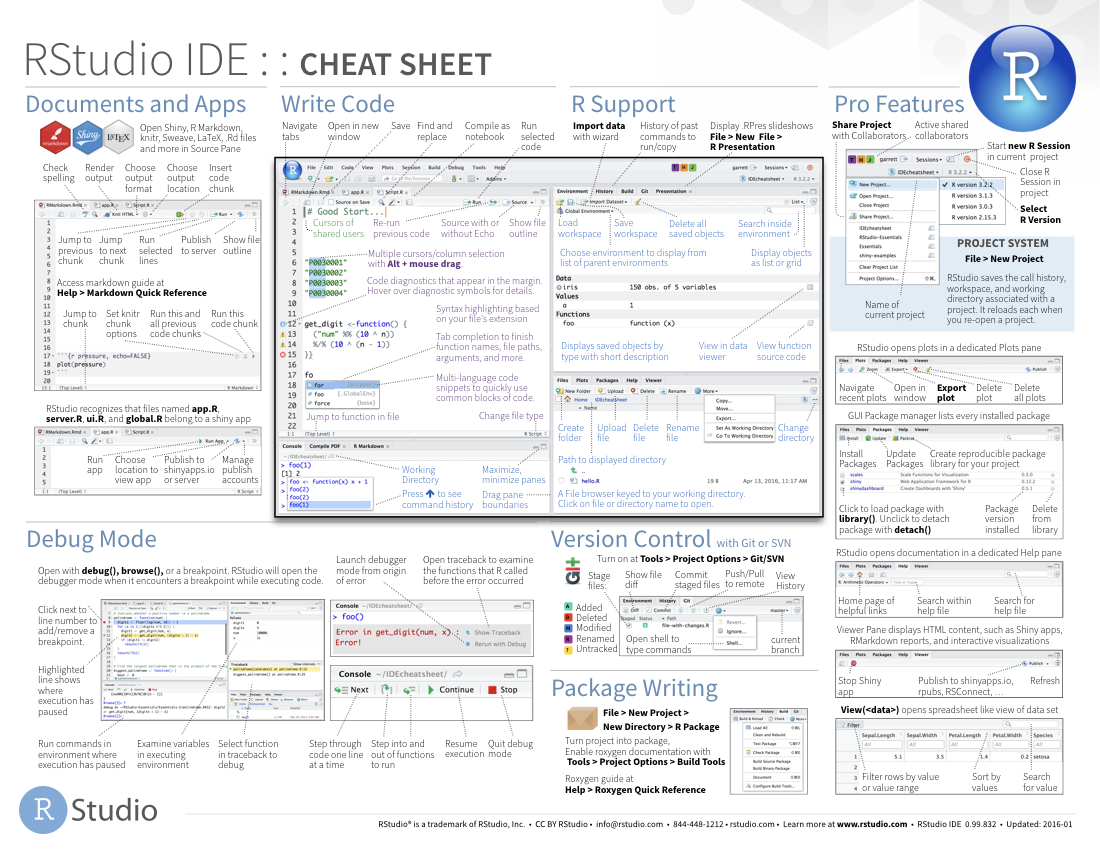
\includegraphics[width=0.8\linewidth]{images/rstudio-ide} 

}

\caption{RStudio Cheat Sheet}\label{fig:rstudio-cheatsheet}
\end{figure}

\section{Supporting Software}\label{supporting-software}

In addition to the above, when writing R code of high complexity or
criticality it is recommended that version control is used:

\begin{itemize}
\tightlist
\item
  \href{http://gitforwindows.org/}{Git} is the market leader and
  integrates well with RStudio. Git is free
\item
  \href{https://www.gitkraken.com/}{GitKraken} provides a very good
  graphical interface to Git and access to more features than RStudio.
  GitKraken is not free, but it does not cost very much.
\end{itemize}

\section{Package Versions}\label{package-versions}

A common problem with R is ensuring everyone is using the same version
of packages. The are a number of ways to deal with this problem:

\begin{enumerate}
\def\labelenumi{\arabic{enumi}.}
\item
  Another approach is to create a site library, a location on a network
  drive where everyone has access to. The default library location can
  then be set to this location so everyone uses the same packages.

  The disadvantage of this approach is that if someone updates a
  packages it is updated for everyone.
\item
  The simplest is to use the
  \href{https://mran.microsoft.com/documents/rro/reproducibility}{checkpoint}
  in Microsoft's R. When installing Microsoft R Open a date is set and
  when packages are installed they are taken from a snapshot of the CRAN
  repository on that date. That way everyone using the same version of
  Microsoft R Open is guaranteed to be using the same version of
  packages.

  The disadvantage of this approach is you cannot use the latest
  features of a package unless the date is brought forward.

  1 and 2 can be combined to avoid installing packages for every user.
\item
  Packrat
\item
  Use Microsoft's
  \href{https://mran.microsoft.com/documents/rro/reproducibility}{\texttt{checkpoint}}
  package to set the date for a piece of work. If a newer version of a
  package is required it can be set in the script and it will be
  downloaded for that bit of work only.

  The disadvantage of this approach is the required packages are
  downloaded separately for each project, so should only be used for
  exceptional cases.
\end{enumerate}

\chapter{Writing R Code}\label{writing}

\section{Writing Style}\label{writing-style}

When writing code it is important to follow a common style so it is
readable and other people, and your future self, can easily understand
and extend it.

\subsection{Tidyverse}\label{tidyverse}

It is recommended, when using R, that we use the
``\href{https://www.tidyverse.org/}{Tidyverse}'' approach and packages
wherever possible. The Tidyverse is a collection of packages designed
for data science, as well as a philosophy and style for formatting data
and writing functions. The
\href{https://www.tidyverse.org/}{tidyverse.org} website details the
packages involved and contains articles on how to use them. Some of it
will be summarised below, but the website contains the definitive
information.

The most in-depth treatment on the Tidyverse can be found in the book
``R for Data Science'', which is available online for free at
\href{http://r4ds.had.co.nz/}{r4ds.had.co.nz}.

The tidyverse has an extensive \href{http://style.tidyverse.org/}{style
guide}, which we summarise here:

\subsection{Files}\label{files}

\begin{itemize}
\tightlist
\item
  File names should be meaningful and end in \texttt{.R}, or
  \texttt{.Rmd} for R markdown files. Only use letters, numbers and
  \texttt{-} or \texttt{\_}.
\item
  If your script required packages load them all at once at the very
  beginning of the file.
\item
  Use comments to explain the ``why'' not the ``what'' or ``how''.
\item
  Break up files into named sections using commented lines
  (\texttt{\#\ -\/-\/-\/-}, example below). In RStudio you can collapse
  and expand sections commented this way.
\end{itemize}

\begin{verbatim}
# Load data --------------------------------------------------------------------
\end{verbatim}

\subsection{Syntax}\label{syntax}

\begin{itemize}
\tightlist
\item
  Variable and function names should use only lowercase letters,
  numbers, and \texttt{\_}.
\item
  Always indent the code inside curly braces \texttt{\{\}} by two
  spaces.
\end{itemize}

\subsection{Functions}\label{functions}

\begin{itemize}
\tightlist
\item
  Use verbs for function names where possible.
\item
  If a function has numerous arguments put each one on a new line.
\item
  A function should do one thing well. If it is doing too much the break
  it up.
\item
  A function should be easily understandable in isolation. It should not
  refer to any variables outside the function scope.
\end{itemize}

\subsection{Pipes}\label{pipes}

\begin{itemize}
\tightlist
\item
  Use \texttt{\%\textgreater{}\%} when you find yourself composing three
  or more functions together, instead of a nested call.
\item
  \texttt{\%\textgreater{}\%} should always have a space before it and a
  new line after it. After the first step, each line should be indented
  by two spaces.
\end{itemize}

\subsection{Documentation}\label{documentation-1}

\begin{itemize}
\tightlist
\item
  Created functions should be documentated so others, including the
  future you, can understand what the function does and how to use it.
\item
  Documentation should be written before the function definition in an
  \href{https://cran.r-project.org/web/packages/roxygen2/vignettes/markdown.html}{roxygen2}
  style. roxygen uses special comments, starting with
  \texttt{\#\textquotesingle{}}. The first line is the title, and
  anything else, not prefixed with a keyword forms the description.
  Keywords start with \texttt{@} and the most important ones are
  \texttt{@param} to describe a function parameter and \texttt{@return}
  to describe what the function returns.
\end{itemize}

Here is a very simple example:

\begin{Shaded}
\begin{Highlighting}[]
\CommentTok{#' The length of a string.}
\CommentTok{#'}
\CommentTok{#' This function returns the number of characters in the supplied string.}
\CommentTok{#' }
\CommentTok{#' @param string input character vector}
\CommentTok{#'}
\CommentTok{#' @return integer vector giving number of characters in each element of the}
\CommentTok{#'   character vector.}
\CommentTok{#'}
\CommentTok{#' @export}
\CommentTok{#'}
\NormalTok{str_length <-}\StringTok{ }\ControlFlowTok{function}\NormalTok{(string) \{}
  \KeywordTok{nchar}\NormalTok{(string)}
\NormalTok{\}}
\end{Highlighting}
\end{Shaded}

\section{Structure}\label{structure}

Organising files for a particular piece of work becomes more important
as the scale and complexity increases. Standard approaches exists to
simplify the workflow.

\subsection{Projects}\label{projects}

Use RStudio projects to organise files. This has a number of advantages:

\begin{enumerate}
\def\labelenumi{\arabic{enumi}.}
\tightlist
\item
  Sets the working directory to the project location
\item
  Reopens the same files when returning to the projects
\end{enumerate}

\subsection{Folders}\label{folders}

When an analysis becomes complex it should be split up into logical
parts and stored in subfolders. Store the original data in a folder,
unchanged. It is better to ``cleanse'' input data with an R script as it
can repeated when data changes, and/or the approach changed itself.

R code may also be stored in a separate folder. You may have an R script
for cleansing the data and another for performing an analysis. Include
an R script at the top level which executes the code in the subfolder in
the appropriate order. Use relative paths to the files. If an RStudio
project has been created the working directory will be set to the
project directory automatically.

Output the results, plots, data, etc, in another folder so it is clear
whether data files are results rather than inputs.

An example of a project structure:

\begin{itemize}
\tightlist
\item
  data

  \begin{itemize}
  \tightlist
  \item
    interesting\_data.xlsx
  \item
    reference\_data.csv
  \end{itemize}
\item
  R

  \begin{itemize}
  \tightlist
  \item
    clean\_data.R
  \item
    analyse.R
  \end{itemize}
\item
  tests

  \begin{itemize}
  \tightlist
  \item
    test\_cleansed\_data.R
  \item
    test\_analysis.R
  \end{itemize}
\item
  results

  \begin{itemize}
  \tightlist
  \item
    cool\_plot.png
  \item
    table\_of\_results.csv
  \end{itemize}
\item
  run\_code.R
\item
  README.md
\end{itemize}

\subsection{README}\label{readme}

Adding a README file is a good way to explain to other, and you future
self, what the analysis does and how to use it. The
\href{index.html\#documentation}{documentation} section of the best
practice has more detail on what should be included.

It is recommended that
\href{http://rmarkdown.rstudio.com/lesson-8.html}{markdown} is used to
write the README. It is a very simple way to specify text formatting in
a plain text file and can be converted to many other formats (HTML,
docx, PDF) if required. In addition, if the package is stored in GitHub
a markdown README is automatically rendered on the repository's page.

\subsection{R Packages}\label{r-packages}

When R code has high criticality consider turning it into a package. A
package is a way of collecting together related code in a robust way. It
has the following advantages:

\begin{itemize}
\tightlist
\item
  Easier to share with others (as a zip file)
\item
  Documentation is compiled into help pages
\item
  All tests can be executed with a single command
\item
  Can implement a development and release process
\item
  Code is broken up into useful functions
\end{itemize}

Writing a package is very straight forward with the helper packages
available today. More information can be found in
\href{packages-development.html}{Package Development}.

\section{R Markdown}\label{r-markdown}

\href{http://rmarkdown.rstudio.com/}{R markdown} is a way of capturing
documentation, code and results and in a single file. The document is
written in plain text using a style called
\href{https://rmarkdown.rstudio.com/authoring_basics.html}{markdown}.
This has a simple syntax for specifying text formatting. R code is added
in ``chunks'' and when the document is rendered the R code is executed
and replaced with the results.

R markdown can be used to produce web pages, Word and PDF documents. The
provide a robust way of capturing an analysis and the results and can be
re-run when the data changes.

RStudio provides a cheatsheet detailing R markdown functionality:

\begin{figure}

{\centering 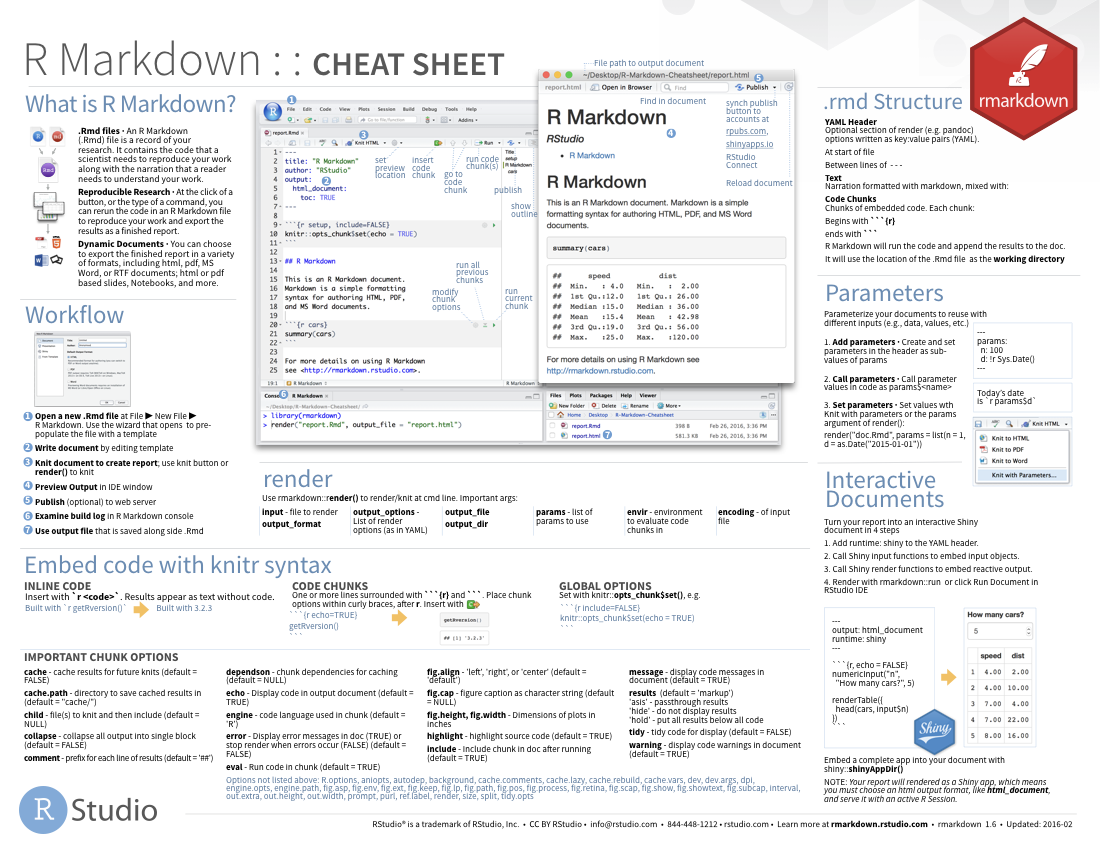
\includegraphics[width=0.8\linewidth]{images/rmarkdown-cheatsheet-2.0} 

}

\caption{R Markdown Cheat Sheet}\label{fig:rmarkdown-cheatsheet}
\end{figure}

\subsection{Markdown}\label{markdown}

Markdown is a lightweight markup language with plain text formatting
syntax. It is designed so that it can be converted to HTML and many
other formats.

\subsubsection{Paragraphs}\label{paragraphs}

Leave at least one empty line between text to start a new paragraph.

\begin{verbatim}
This is the first paragraph.

This is the second paragraph.
\end{verbatim}

This is the first paragraph.

This is the second paragraph.

\subsubsection{Headers}\label{headers}

\begin{verbatim}
# Header 1

## Header 2

### Header 3
\end{verbatim}

\subsubsection{Emphasis}\label{emphasis}

\begin{verbatim}
*italic*   **bold**

_italic_   __bold__
\end{verbatim}

\emph{italic} \textbf{bold}

\emph{italic} \textbf{bold}

\subsubsection{Lists}\label{lists}

Unordered List:

\begin{verbatim}
* Item 1
* Item 2
    + Item 2a
    + Item 2b
\end{verbatim}

\begin{itemize}
\tightlist
\item
  Item 1
\item
  Item 2

  \begin{itemize}
  \tightlist
  \item
    Item 2a
  \item
    Item 2b
  \end{itemize}
\end{itemize}

Ordered List:

\begin{verbatim}
1. Item 1
2. Item 2
3. Item 3
    a. Item 3a
    b. Item 3b
\end{verbatim}

\begin{enumerate}
\def\labelenumi{\arabic{enumi}.}
\tightlist
\item
  Item 1
\item
  Item 2
\item
  Item 3

  \begin{enumerate}
  \def\labelenumii{\alph{enumii}.}
  \tightlist
  \item
    Item 3a
  \item
    Item 3b
  \end{enumerate}
\end{enumerate}

\subsubsection{Links}\label{links}

Use a plain http address or add a link to a phrase:

\begin{verbatim}
http://example.com

[linked phrase](http://example.com)
\end{verbatim}

\url{http://example.com}

\href{http://example.com}{linked phrase}

\subsubsection{Images}\label{images}

Images on the web or local files in the same directory:

\begin{verbatim}
![](https://upload.wikimedia.org/wikipedia/commons/1/1b/R_logo.svg)

![optional caption text](images/octocat.png)
\end{verbatim}

\begin{figure}
\centering

\includegraphics{images/R_logo.png}
\caption{}
\end{figure}

\begin{figure}
\centering

\includegraphics{images/octocat.png}
\caption{optional caption text}
\end{figure}

\subsubsection{Reference Style Links and
Images}\label{reference-style-links-and-images}

Links

\begin{verbatim}
A [linked phrase][id].

At the bottom of the document:

[id]: http://example.com/ "Title"
\end{verbatim}

A \href{images/octocat.png}{linked phrase}.

At the bottom of the document:

Images

\begin{verbatim}
![alt text][id]

At the bottom of the document:

[id]: images/octocat.png "Octocat"
\end{verbatim}

\begin{figure}
\centering

\includegraphics{images/octocat.png}
\caption{alt text}
\end{figure}

At the bottom of the document:

\subsubsection{Blockquotes}\label{blockquotes}

\begin{verbatim}
A friend once said:

> It's always better to give
> than to receive.
\end{verbatim}

A friend once said:

\begin{quote}
It's always better to give than to receive.
\end{quote}

\subsubsection{Plain Code Blocks}\label{plain-code-blocks}

Plain code blocks are displayed in a fixed-width font but not evaulated

\begin{verbatim}
```
This text is displayed verbatim / preformatted
```
\end{verbatim}

\begin{verbatim}
This text is displayed verbatim / preformatted
\end{verbatim}

\subsubsection{Inline Code}\label{inline-code}

\begin{verbatim}
We defined the `add` function to compute the sum of two numbers.
\end{verbatim}

We defined the \texttt{add} function to compute the sum of two numbers.

\subsubsection{LaTeX Equations}\label{latex-equations}

Inline equation:

\begin{verbatim}
Einstein's famous equation $E = mc^2$
\end{verbatim}

Einstein's famous equation \(E = mc^2\)

Display equation:

\begin{verbatim}
$$
E = mc^2
$$
\end{verbatim}

\[
E = mc^2
\]

\subsubsection{Horizontal Rule / Page
Break}\label{horizontal-rule-page-break}

Three or more asterisks or dashes:

\begin{verbatim}
******

------
\end{verbatim}

\begin{center}\rule{0.5\linewidth}{\linethickness}\end{center}

\begin{center}\rule{0.5\linewidth}{\linethickness}\end{center}

\subsubsection{Tables}\label{tables}

\begin{verbatim}
First Header  | Second Header
------------- | -------------
Content Cell  | Content Cell
Content Cell  | Content Cell
\end{verbatim}

\begin{longtable}[]{@{}ll@{}}
\toprule
First Header & Second Header\tabularnewline
\midrule
\endhead
Content Cell & Content Cell\tabularnewline
Content Cell & Content Cell\tabularnewline
\bottomrule
\end{longtable}

\subsubsection{Manual Line Breaks}\label{manual-line-breaks}

End a line with a backslash:

\begin{verbatim}
Roses are red,\
Violets are blue.
\end{verbatim}

Roses are red,\\
Violets are blue.

\subsubsection{Miscellaneous}\label{miscellaneous}

\begin{verbatim}
superscript^2^

~~strikethrough~~
\end{verbatim}

superscript\textsuperscript{2}

\sout{strikethrough}

\subsection{R Markdown}\label{r-markdown-1}

\subsubsection{R Code Chunks}\label{r-code-chunks}

R code will be evaluated and printed

\begin{Shaded}
\begin{Highlighting}[]
\KeywordTok{summary}\NormalTok{(cars}\OperatorTok{$}\NormalTok{dist)}
\end{Highlighting}
\end{Shaded}

\begin{verbatim}
##    Min. 1st Qu.  Median    Mean 3rd Qu.    Max. 
##    2.00   26.00   36.00   42.98   56.00  120.00
\end{verbatim}

\begin{Shaded}
\begin{Highlighting}[]
\KeywordTok{summary}\NormalTok{(cars}\OperatorTok{$}\NormalTok{speed)}
\end{Highlighting}
\end{Shaded}

\begin{verbatim}
##    Min. 1st Qu.  Median    Mean 3rd Qu.    Max. 
##     4.0    12.0    15.0    15.4    19.0    25.0
\end{verbatim}

Inline R Code

There were 50 cars studied

\subsection{R Notebooks}\label{r-notebooks}

\chapter{Recommended Packages}\label{packages}

\section{Data Wrangling}\label{data-wrangling}

\begin{quote}
Data wrangling is the process of transforming and mapping data from one
``raw'' data form into another format with the intent of making it more
appropriate and valuable for a variety of downstream purposes such as
analytics.

-- \href{https://en.wikipedia.org/wiki/Data_wrangling}{\emph{Wikipedia}}
\end{quote}

\subsection{Tidy Data}\label{tidy-data}

The Tidyverse of packages are built around the concept of tidy data,
first introduced by Jeff Leek in his book \emph{The Elements of Data
Analytic Style}. Hadley Wickham summarises the characteristics of
\href{http://tidyr.tidyverse.org/articles/tidy-data.html}{tidy data}
with the following points:

\begin{enumerate}
\def\labelenumi{\arabic{enumi}.}
\tightlist
\item
  Each variable forms a column.
\item
  Each observation forms a row.
\item
  Each type of observational unit forms a table.
\end{enumerate}

\subsection{Cheatsheets}\label{cheatsheets}

RStudio provide a selection of cheatsheets containing quick reference of
R functions useful for common task:

\begin{figure}

{\centering 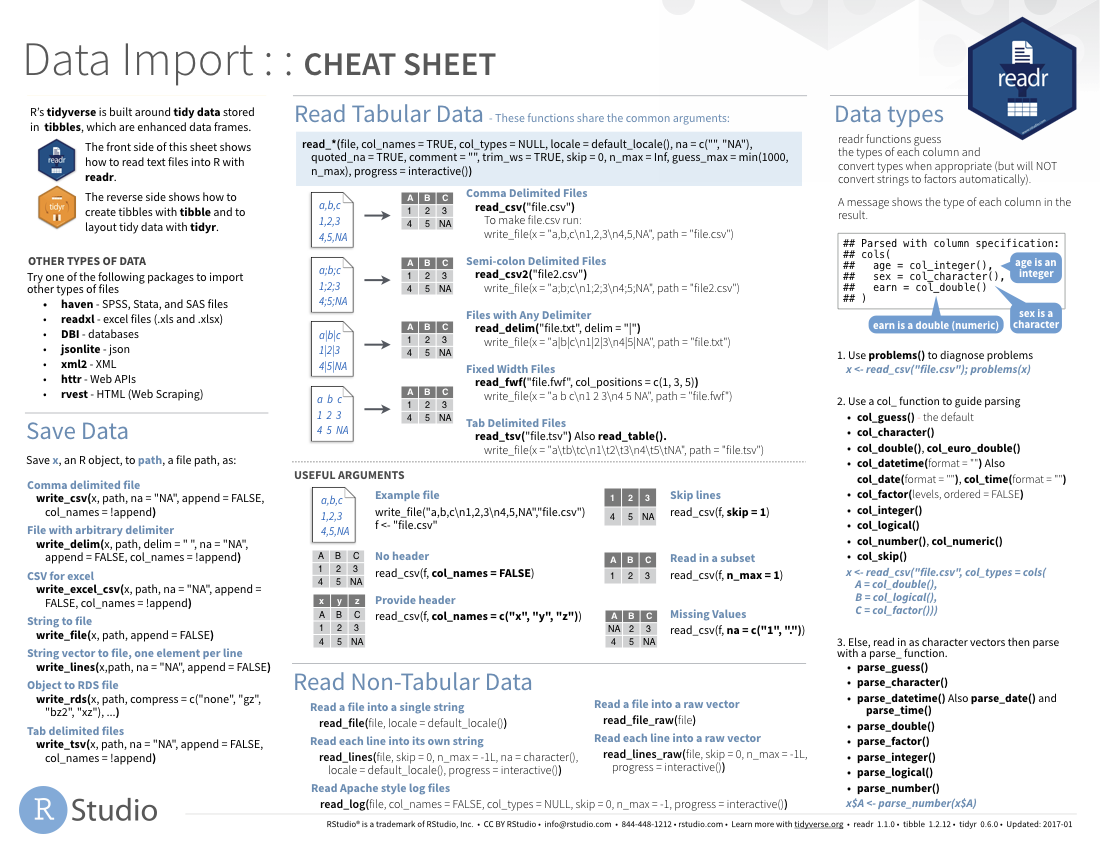
\includegraphics[width=0.8\linewidth]{images/data-import-cheatsheet-1} 

}

\caption{Data Import}\label{fig:data-import-cheatsheet}
\end{figure}

\begin{figure}

{\centering 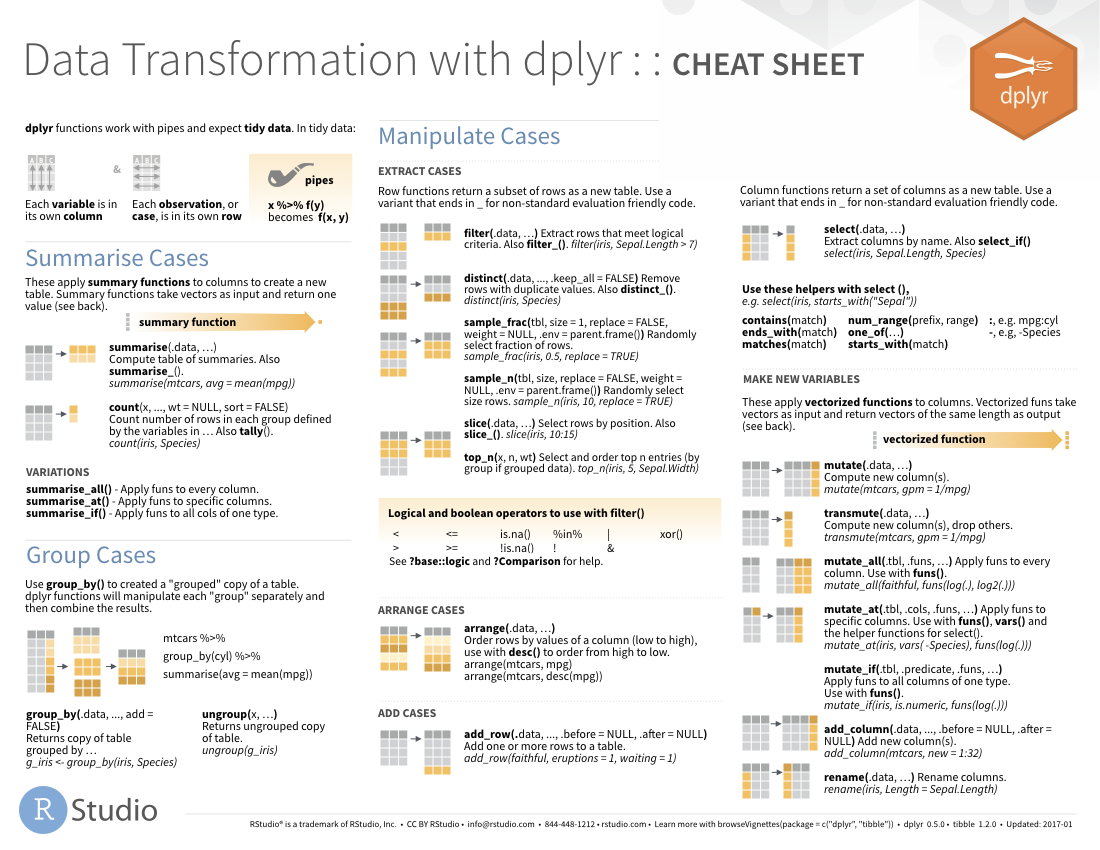
\includegraphics[width=0.8\linewidth]{images/data-transformation-cheatsheet} 

}

\caption{Data Transformation}\label{fig:data-transformation-cheatsheet}
\end{figure}

\begin{figure}

{\centering 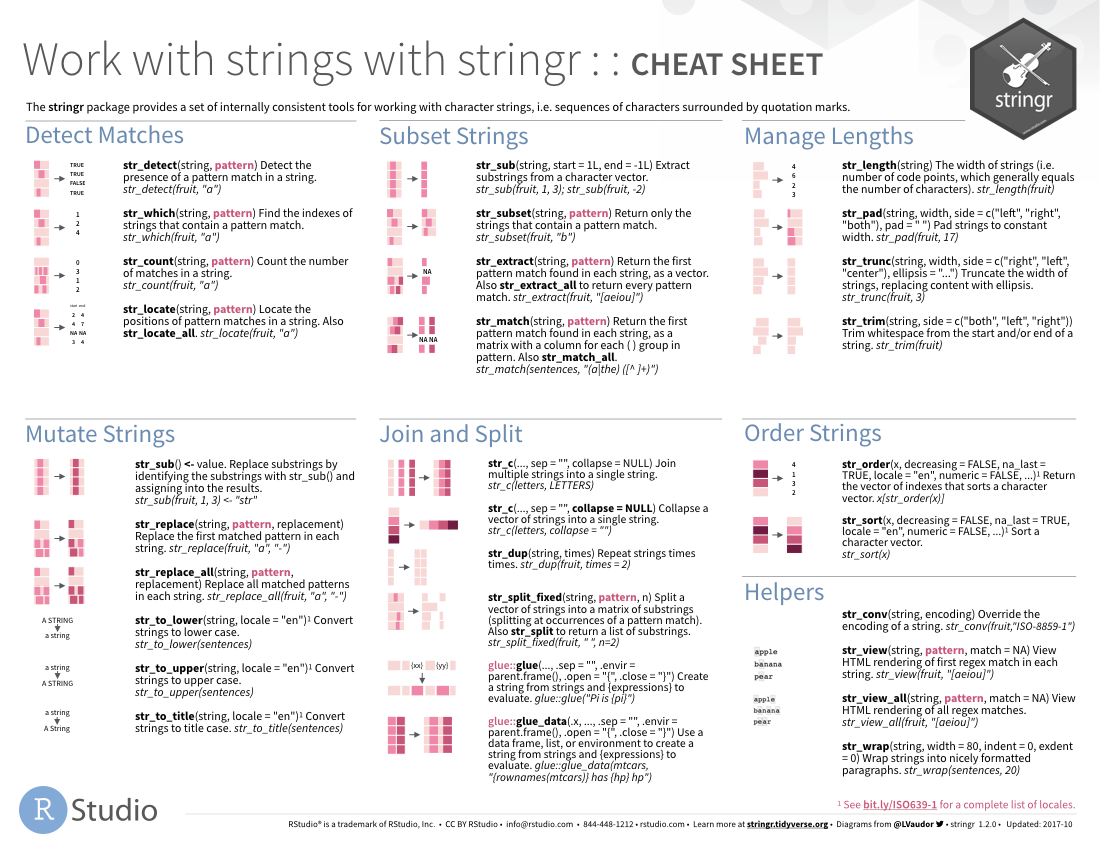
\includegraphics[width=0.8\linewidth]{images/strings} 

}

\caption{Strings}\label{fig:strings-cheatsheet}
\end{figure}

\begin{figure}

{\centering 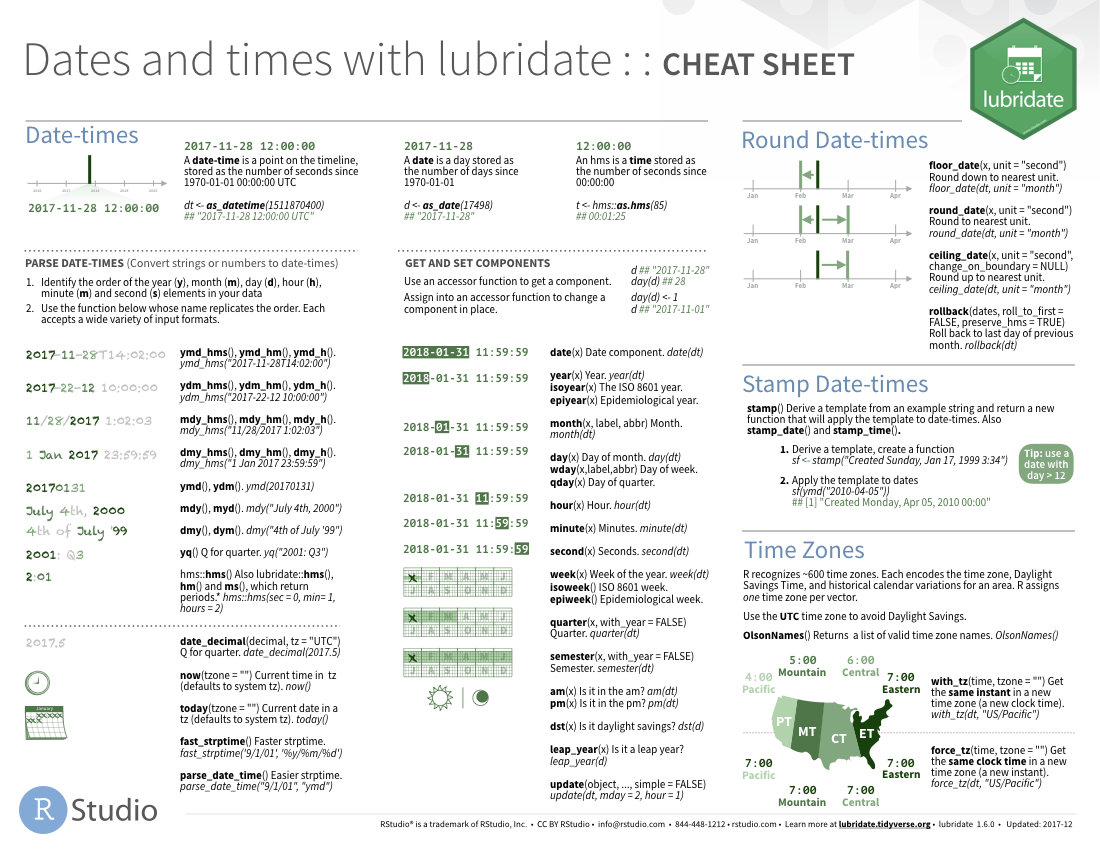
\includegraphics[width=0.8\linewidth]{images/lubridate} 

}

\caption{Dates and Times}\label{fig:lubridate-cheatsheet}
\end{figure}

\subsection{Importing Data}\label{importing-data}

The first step in wrangling is importing the data into R. The methods to
do so depend on the source of data:

\begin{itemize}
\tightlist
\item
  Reading files
\item
  Connecting to databases
\item
  Web APIs or pages
\end{itemize}

\subsubsection{Reading Files}\label{reading-files}

Files may come in many formats and R has packages to read many of them.
The most common for data science are tabular text files, such as CSVs,
and Excel spreadsheets. The recommended packages for reading these files
are:.

\begin{itemize}
\tightlist
\item
  \href{http://readr.tidyverse.org/}{\texttt{readr}} for reading text
  files
\item
  \href{http://readxl.tidyverse.org/}{\texttt{readxl}} for reading Excel
  files
\item
  \href{https://www.rdocumentation.org/packages/openxlsx/}{\texttt{openxlsx}}
  for writing to Excel files
\end{itemize}

\subsubsection{Connecting to Databases}\label{connecting-to-databases}

The new \href{https://db.rstudio.com/}{RStudio Connections Pane} makes
it possible to easily connect to a variety of data sources, and explore
the objects and data inside the connection.

The recommended packages for connecting to databases (also used by
RStudio) are:

\begin{itemize}
\tightlist
\item
  \href{https://db.rstudio.com/DBI}{\texttt{DBI}} provides a standard
  interface to any database
\item
  \href{https://db.rstudio.com/odbc/}{\texttt{odbc}} for connecting to
  databases using ODBC
\item
  \href{https://db.rstudio.com/dplyr/}{\texttt{dplyr}} for transforming
  tables in a database
\end{itemize}

\subsubsection{Web APIs and Pages}\label{web-apis-and-pages}

Obtaining data from the internet has two main approaches. If the website
provides an application programming interface (API) then you can send
and receive data through it. The data from web APIs is usually returned
in JSON or XML format. Alternatively, you can scrape the website itself,
extracting data from the pages. The recommended packages for these
approaches are:

\begin{itemize}
\tightlist
\item
  \href{http://httr.r-lib.org/}{\texttt{httr}} for communicating with
  web APIs
\item
  \href{https://www.rdocumentation.org/packages/jsonlite}{\texttt{jsonlite}}
  for reading JSON formatted text
\item
  \href{https://www.rdocumentation.org/packages/xml2}{\texttt{xml2}} for
  reading XML formatted text
\item
  \href{https://www.rdocumentation.org/packages/rvest}{\texttt{rvest}}
  for scraping web pages
\end{itemize}

\subsection{Tidying Data}\label{tidying-data}

Now you have the data you want, it probably requires some processing in
order to get it into a structure that is useful for analysis. There are
two main packages for this
\href{http://tidyr.tidyverse.org}{\texttt{tidyr}} and
\href{http://dplyr.tidyverse.org}{\texttt{dplyr}}:

\subsubsection{\texorpdfstring{\href{http://tidyr.tidyverse.org}{\texttt{tidyr}}}{tidyr}}\label{tidyr}

The focus of \href{http://tidyr.tidyverse.org}{\texttt{tidyr}} is to get
the data into a tidy format. The main functions it provides to do this
are:

\begin{itemize}
\tightlist
\item
  \href{http://tidyr.tidyverse.org/reference/gather.html}{\texttt{gather()}}
  takes multiple columns, and gathers them into key-value pairs: it
  makes ``wide'' data longer.
\item
  \href{http://tidyr.tidyverse.org/reference/spread.html}{\texttt{spread()}}
  takes two columns (key \& value) and spreads in to multiple columns,
  it makes ``long'' data wider.
\item
  \href{http://tidyr.tidyverse.org/reference/separate.html}{\texttt{separate()}}
  and
  \href{http://tidyr.tidyverse.org/reference/extract.html}{\texttt{extract()}}
  pulls apart a column that represents multiple variables.
\item
  \href{http://tidyr.tidyverse.org/reference/unite.html}{\texttt{unite()}}
  combines columns, useful if one is redundant.
\item
  \href{http://tidyr.tidyverse.org/reference/gather.html}{\texttt{separate\_rows()}}
  for separating a row that contains multiple observations.
\end{itemize}

In addition, \href{http://tidyr.tidyverse.org}{\texttt{tidyr}} provides
a set of functions for dealing with implicit and explicit missing
values:

\begin{itemize}
\tightlist
\item
  \href{http://tidyr.tidyverse.org/reference/drop_na.html}{\texttt{drop\_na()}}:
  Drop rows containing missing values
\item
  \href{http://tidyr.tidyverse.org/reference/replace_na.html}{\texttt{replace\_na()}}:
  Replace missing values
\item
  \href{http://tidyr.tidyverse.org/reference/fill.html}{\texttt{fill()}}:
  Fill in missing values.
\item
  \href{http://tidyr.tidyverse.org/reference/complete.html}{\texttt{complete()}}:
  Complete a data frame with missing combinations of data.
\item
  \href{http://tidyr.tidyverse.org/reference/expand.html}{\texttt{expand()}},
  \href{http://tidyr.tidyverse.org/reference/expand.html}{\texttt{crossing()}}:
  Expand data frame to include all combinations of values
\end{itemize}

\subsubsection{\texorpdfstring{\href{http://dplyr.tidyverse.org}{\texttt{dplyr}}}{dplyr}}\label{dplyr}

\href{http://dplyr.tidyverse.org}{\texttt{dplyr}} is a grammar of data
manipulation, providing a consistent set of verbs that help you solve
the most common data manipulation challenges:

\begin{itemize}
\tightlist
\item
  \href{http://dplyr.tidyverse.org/reference/mutate.html}{\texttt{mutate()}}
  adds new variables that are functions of existing variables.
\item
  \href{http://dplyr.tidyverse.org/reference/select.html}{\texttt{select()}}
  picks variables based on their names.
\item
  \href{http://dplyr.tidyverse.org/reference/filter.html}{\texttt{filter()}}
  picks cases based on their values.
\item
  \href{http://dplyr.tidyverse.org/reference/summarise.html}{\texttt{summarise()}}
  reduces multiple values down to a single summary.
\item
  \href{http://dplyr.tidyverse.org/reference/arrange.html}{\texttt{arrange()}}
  changes the ordering of the rows.
\end{itemize}

These all combine naturally with
\href{http://dplyr.tidyverse.org/reference/group_by.html}{\texttt{group\_by()}}
which allows you to perform any operation ``by group''.

\href{http://dplyr.tidyverse.org}{\texttt{dplyr}} also provides a set of
functions for combining tables. Mutating joins combine tables based on
matching a subset of common variables; Set operations expect the tables
to have the same variables and combine observations like sets.

\textbf{Mutating joins}

\begin{itemize}
\tightlist
\item
  \href{http://dplyr.tidyverse.org/reference/join.html}{\texttt{inner\_join(x,\ y)}}
  only includes observations that match in both \texttt{x} and
  \texttt{y}.
\item
  \href{http://dplyr.tidyverse.org/reference/join.html}{\texttt{left\_join(x,\ y)}}
  includes all observations in \texttt{x}, regardless of whether they
  match or not.
\item
  \href{http://dplyr.tidyverse.org/reference/join.html}{\texttt{right\_join(x,\ y)}}
  includes all observations in \texttt{y}. It's equivalent to
  \href{http://dplyr.tidyverse.org/reference/join.html}{\texttt{left\_join(y,\ x)}},
  but the columns will be ordered differently.
\item
  \href{http://dplyr.tidyverse.org/reference/join.html}{\texttt{full\_join()}}
  includes all observations from \texttt{x} and \texttt{y}.
\end{itemize}

\textbf{Set operations}

\begin{itemize}
\tightlist
\item
  \href{http://dplyr.tidyverse.org/reference/setops.html}{\texttt{intersect(x,\ y)}}:
  returns only observations in both \texttt{x} and \texttt{y}.
\item
  \href{http://dplyr.tidyverse.org/reference/setops.html}{\texttt{union(x,\ y)}}:
  returns unique observations in \texttt{x} and \texttt{y}.
\item
  \href{http://dplyr.tidyverse.org/reference/setops.html}{\texttt{setdiff(x,\ y)}}:
  return observations in \texttt{x}, but not in \texttt{y}.
\end{itemize}

\subsubsection{Variable Types}\label{variable-types}

There are also packages which simplify working with specific types of
data:

\begin{itemize}
\tightlist
\item
  \href{http://stringr.tidyverse.org/}{\texttt{stringr}} for strings and
  regular expressions
\item
  \href{http://forcats.tidyverse.org/}{\texttt{forcats}} for factors,
  used to handle categorical data
\item
  \href{http://lubridate.tidyverse.org/}{\texttt{lubridate}} for dates
  and date-times.
\item
  \href{https://www.rdocumentation.org/packages/hms}{\texttt{hms}} for
  time-of-day values.
\end{itemize}

\subsubsection{\texorpdfstring{\href{http://tibble.tidyverse.org/}{\texttt{tibble}}}{tibble}}\label{tibble}

When using these packages you may notice they return a \texttt{tibble}
rather than a \texttt{data.frame}. They are basically the same thing
with three key differences:

\begin{enumerate}
\def\labelenumi{\arabic{enumi}.}
\tightlist
\item
  Printing: Tibbles only show the first ten rows and all the columns
  that fit on one screen.
\item
  Subsetting: \texttt{{[}} always returns another tibble. \texttt{\$}
  never uses partial matching.
\item
  Recycling: Only values of length 1 are recycled. Trying to combine
  columns of different length throws an error.
\end{enumerate}

The package \href{http://tibble.tidyverse.org/}{\texttt{tibble}} has
some useful functions for constructing tibbles. In particaular, you can
construct a tibble row-wise using the
\href{http://tibble.tidyverse.org/reference/tribble.html}{\texttt{tribble}}
function (transposed tibble).

\bibliography{book.bib,packages.bib}


\end{document}
